% Revisão OK 09/10
\chapter{Decodificação do METAR}

O METAR é um protocolo de transmissão de dados meteorológicos de um aeroporto ou 
aeródromo \cite{metar-what}. Não se trata de uma previsão do tempo, mas sim de uma visualização atual. 
Para previsões existe o TAF que será explorado no próximo capítulo.
O METAR é formado por itens separados por espaço. Cada item corresponde a uma 
unidade mínima de informação meteorológica. Com os dados de sensores instalados 
no aeródromo \cite{metar-weather-gov}, a cada hora é publicado um novo METAR que
é válido para aquela hora. Em casos excepcionais, quando as condições de tempo 
estiverem mudando repentinamente, um METAR pode ser atualizado a cada meia hora
 \cite{METAR-speci} ou menos, o autor já viu o METAR do aeroporto do Galeão sendo atualizado
 na hora cheia e depois no minuto 16. Nas próximas seções, será apresentado um 
 exemplo de METAR e sua decodificação bem como uma explicação do algorítmo.

\section{Exemplo}
O METAR no aeroporto de Fortaleza (Pinto Martins)\cite{METAR-sbfz}, no dia 17 de 
abril de 2024 às 10:54 foi

\texttt{SBFZ 171300Z 15010KT 9999 BKN019 SCT025 FEW030TCU BKN100 30/25 Q1011}.

"SBFZ" se refere ao código ICAO (\textit{International Civil Aviation Organization}) do 
aeroporto, não confundir com o código IATA (\textit{International Air Transport Association}) 
que é formado por três letras. O aeroporto Pinto Martins possui o código IATA FOR, 
o Santos Dumont SDU e o Galeão GIG. O público leigo parece conhecer mais este 
código, mas na aviação costuma-se usar mais o código ICAO, pois \textit{todos} os 
aeródromos possuem um, enquanto o IATA só é presente em aeroportos onde há 
processamento de bagagem \cite{iata-codes} \cite{icao-codes}.

\begin{itemize}
\item \textbf{171300Z} significa que este METAR se refere ao dia 17 às 13 horas e zero 
minuto zulu. Horário zulu é simplesmente o fuso horário da longitude de zero grau, 
chamado de hora UTC ou Coordinated Universal Time \cite{UTC}. Para que não haja 
confusão com fusos horários, a aviação usa o horário UTC. Em tempo
estável, este 
METAR será válido até às 13:59, quando será substituído pelo METAR iniciando com 
"SBFZ 171400Z". Pode haver alteração antes em caso de mudança repentina de condições 
atmosféricas.

Note-se que a seguinte expressão regular com três grupos de captura consegue extrair 
o dia, a hora e o minuto:

\begin{verbatim}
([0-9]{2})([0-9]{2})([0-9]{2})Z
\end{verbatim}

Com o METAR supracitado, os grupos de captura serão:

\begin{itemize}
\item Grupo 1 (dia): 17
\item Grupo 2 (hora): 13
\item Grupo 3 (minuto): 00
\end{itemize}

\item \textbf{15010KT} se refere à velocidade e direção do vento. Os três primeiros 
algarismos informam a direção na bússola, em graus, de onde o vento sopra, e os 
últimos dois algarismos informam a velocidade do vento em nós (milhas náuticas por hora). 
Neste caso, o vento vem da direção 150 graus com velocidade de dez nós. Com a 
expressão abaixo extraímos essas duas informações:

\begin{verbatim}
([0-9]{3})([0-9]{2})KT
\end{verbatim}

A informação de vento pode também conter a letra G (gust) para rajadas e a letra 
V (variable) em um item separado para o caso de haver variação de direção. Por 
exemplo, um METAR com os itens \texttt{10016G21KT 080V120} informa que há rajadas 
de até 21 kt e a direção do vento pode variar de 80 a 120 graus. Existem outros 
aeroportos que podem usar outras unidades para a velocidade do vento, mas no 
Brasil só é usado nós (kt). Para obter essas informações usamos o regex 
\verb|([0-9]{3}[0-9]{2}G{[0-9]{2}}) e \verb|([0-9]{3})V([0-9]{3})|.

\item \textbf{9999} significa visibilidade ilimitada (maior ou igual a 10 km). Se fosse 
6000, a visibilidade seria de 
6 km. Por ser sempre quatro algarismos, o regex \verb|([0-9]{4})| consegue capturar 
essa informação.

\item \textbf{30/25} Temperatura 30°C e ponto de orvalho 25°C. Caso a temperatura seja 
negativa, a letra M é adicionada antes do número. M2/M5 significa temperatura 
-2°C e ponto de orvalho -5°C \cite{METAR-help}. O regex usado é

\texttt{(M?[0-9]{2})/(M?[0-9]{2})}

Observe o M opcional. É necessário depois fazer a substituição do M para o sinal
de menos.

\item \textbf{Q1012} O altímetro do avião deve ser ajustado para 1012 hectopascal. 
Também pode ser usada a unidade polegadas de mercúrio (mmHg), mas no Brasil esta 
não é usada no METAR. O regex é\verb|(Q[0-9]{4})|

\item \textbf{SCT025} Nuvens espalhadas (3/8 a 4/8 do céu com nuvens) em 2500 pés de 
altitude. 025 se refere ao nível de voo (Flight Level), que é a altitude acima 
do nível médio do mar com divisão exata por 100.

\item \textbf{FEW030TCU} Poucas nuvens (1/8 a 2/8 do céu com nuvens) em 3000 pés de 
altitude. O sufixo TCU significa que há nuvens convectivas significativas \cite{decea-mil}.

\item \textbf{BKN100} Nuvens broken (5/8 a 7/8 do céu com nuvens) em 10000 pés de altitude.

Existe também o tipo OVC (overcast) que se refere a totalmente encoberto. O regex 
usado é \verb|([A-Z]{3})([0-9]{3})(TCU)?|. O primeiro grupo de captura é comparado 
com "FEW", "BKN", "SCT" e "OVC".

\end{itemize}

\section{Algoritmo}

O objetivo do módulo de decoder é dar uma explicação automática semelhante a esta 
para qualquer tipo de METAR de aeroportos no Brasil. O módulo usa várias expressões 
regulares para decodificar uma grande quantidade de informações, porém não é exaustivo; 
foi dada preferência a fenômenos que podem ocorrer no Brasil \cite{decea-mil}.

O algoritmo deve separar a string do METAR pelo caractere de espaço. Para cada 
item separado, cada expressão regular é testada, não é garantida uma ordem dos itens.
 Caso uma combinação ocorra, os grupos de captura são interpolados em uma string 
 que explica aquele item. 

\section{Exemplo}

Sendo "\$1" o primeiro grupo de captura, "\$2" o segundo e "\$3" o terceiro, o item "27008G16KT", 
por exemplo é comparado com todas as expressões regex e ocorre o match com apenas a seguinte:

\begin{verbatim}
  ([0-9]\{3\})([0-9]\{2\})G([0-9]\{2\})KT
\end{verbatim}

que é mapeada para a frase

\begin{verbatim}
  Vento \$1° com \$2 nós e rajadas de até \$3 nós
\end{verbatim}

com os grupos de captura do regex supracitado. Então, será gerada uma tupla
\texttt{(27008G16KT, Vento 270° com 8 nós e rajadas de até 16 nós)}. O retorno do 
algoritmo será uma lista de tuplas enviada à ferramenta de templating
de página Jinja.

A seguir um exemplo para esta lista de tuplas:

\lstinputlisting[label=rett:metar, language=Python]{code/metar.json}

E como é mostrado na página:

\begin{figure}[ht]
  \begin{center}
  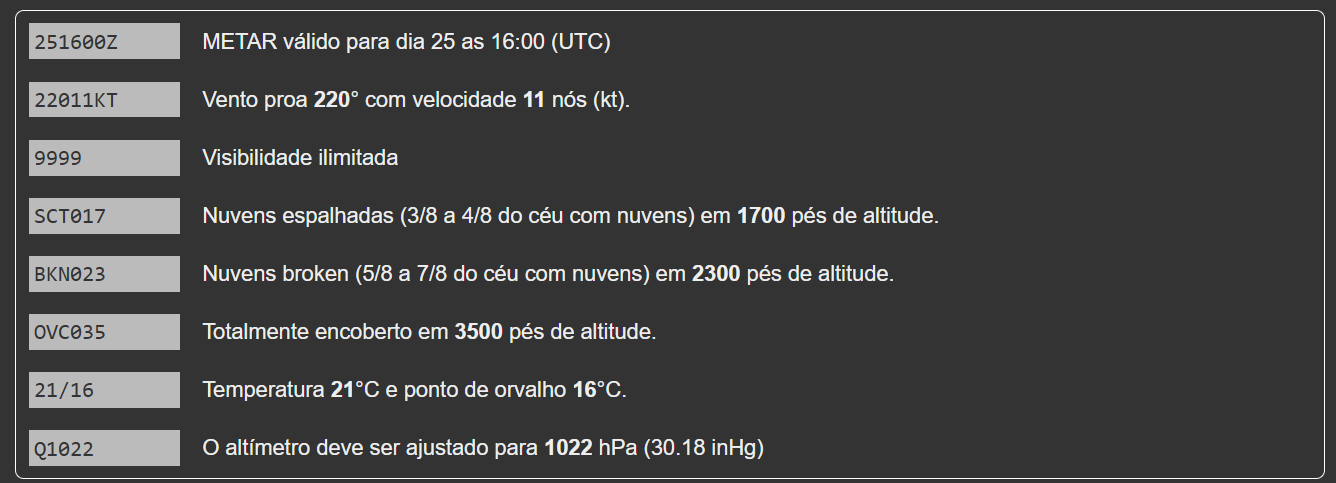
\includegraphics[width=400pt]{img/metar-sbgl.png}
  \caption{METAR do aeroporto do Galeão dia 30 de agosto de 2024}
  \label{fig:metar-30-08}
  \end{center}
\end{figure}
